\subsection{SVD: Singular Value Decomposition}
In linear algebra, the singular value decomposition (SVD) is a factorization of
a real or complex matrix. It generalizes the eigendecomposition of a square normal
matrix with an orthonormal eigenbasis to any {m X n} matrix.
\footnote{\href{https://en.wikipedia.org/wiki/Singular\_value\_decomposition}{https://en.wikipedia.org/wiki/Singular\_value\_decomposition}}\\
In terms of a Movie Recommender System, the SVD decreases the dimension of the utility matrix
by extracting its latent factors (e.g.: age, humour, etc.), and generating an accessible way of
comparing movies and users.\\
\begin{center}
    \captionsetup{type=figure}
    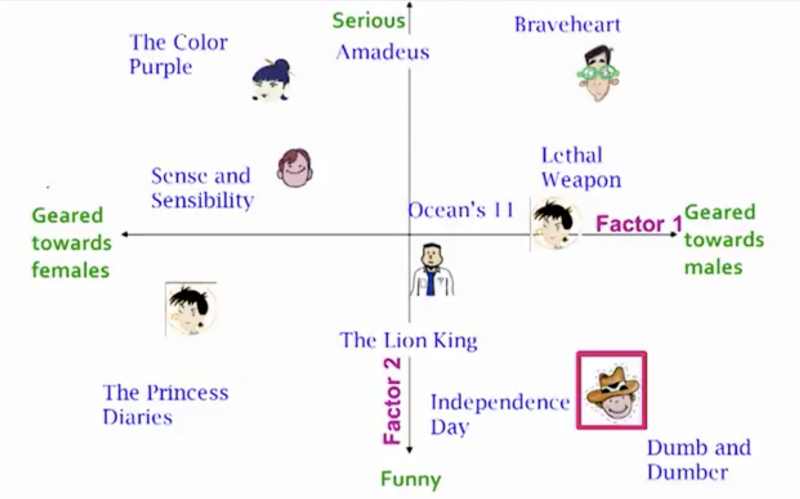
\includegraphics[width=250px]{images/svd-00.png}
    \captionof{figure}{Movie-User simplified-by-SVD comparison}
\end{center}
\subsubsection*{Implementation}
We use the library Surprise\footnote{\href{https://surprise.readthedocs.io/en/stable/matrix\_factorization.html}{https://surprise.readthedocs.io/en/stable/matrix\_factorization.html}}
for implementing our solution. We separate the problem in four different "modules", each one of them represented by a function
and (in most cases) depending on the others:
\begin{enumerate}
    \item Generate SVD model
    \item Predict a score (given a user and a movie)
    \item Get predictions for all movies previously rated in the system (given a user)
    \item Get top predictions
\end{enumerate}
\subsubsection*{Generate Model}
Generating and fitting the model is simplified to us by the library itself.
The cross-validation of training it with our smaller dataset gives us the following results for RSME (Root Mean Square Error) and MAE (Mean Average Error):\\
\begin{center}
    \captionsetup{type=figure}
    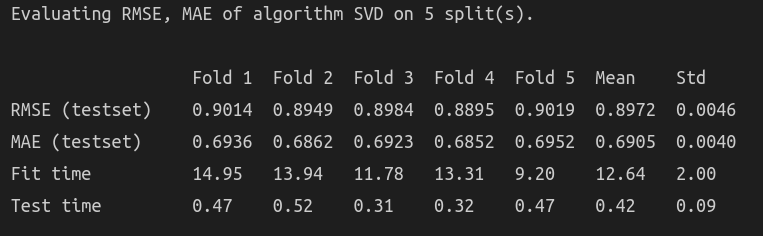
\includegraphics[width=250px]{images/svd-val.png}
    \captionof{figure}{SVD cross-validation}
\end{center}
After making it fit our data, we serialize the generated model using \emph{joblib}
\footnote{\href{https://joblib.readthedocs.io/en/latest/generated/joblib.dump.html}{https://joblib.readthedocs.io/en/latest/generated/joblib.dump.html}},
and from now on we don't need to generate it anymore, but just deserialize it and use it.
\subsubsection*{Predict one score}
Predicting a score involves sending a user and a movie to the SVD model and getting a predicted score (between 1 and 5) for the pair.
For example, asking for the estimate of the score for the movie of id 3 likely given by the user 3 returns us a Prediction object like the following (being \emph{est} the predicted value):
\begin{center}
    \emph{Prediction(uid=3, iid=3, r\_ui=None, est=3.154562267959806, details={'was\_impossible': False})}
\end{center}
\subsubsection*{Predict scores for every movie}
The previous step gives us way to the next one:
if we want to recommend top movies for one user, we can apply the SVD predictor to all rated movies (not by our user) within our dataset
and assign them a potential score for each user-movie pair.
For an increasing dataset, the latter process is batch-intensive, and that's why we use the concurrent.futures\footnote{\href{https://docs.python.org/3/library/concurrent.futures.html}{https://docs.python.org/3/library/concurrent.futures.html}}
Python standard library for running each prediction concurrently.
Applying this process we obtain a list of pairs \emph{(movie id, prediction object)}.
% TODO: talk about caching this list
\subsubsection*{Get top predictions}
Finally, we use this list, order it by prediction value (descending) and take the best 10 movies as our final result.
\begin{center}
    \captionsetup{type=figure}
    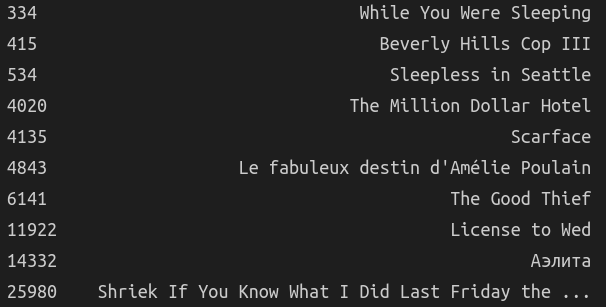
\includegraphics[width=250px]{images/svd-top.png}
    \captionof{figure}{SVD: top 10 predictions for user}
\end{center}